\documentclass[sigconf,nonacm]{acmart}
\usepackage{amsmath,booktabs,tikz,pgfplots}
\pgfplotsset{compat=1.18}
\setlength{\emergencystretch}{3em}
\settopmatter{printacmref=false,printfolios=true}
\renewcommand\footnotetextcopyrightpermission[1]{}
\title{Attacker Memory Changes Deception Policy Rankings: An Audited Simulator Study of Offline Selection}
\author{Ezekiel Ologunde}
\affiliation{\institution{Independent Researcher}\city{Boston}\state{MA}\country{USA}}
\email{ologunde@bu.edu}
\begin{document}
\begin{abstract}
Deception evaluations can reset attacker knowledge between encounters even when a deployed opponent would retain successful target identities. We study the resulting policy-selection sensitivity in a controlled Cyberwheel simulator experiment. Three equal-budget stochastic decoy-placement policies are compared under reset and retained attacker memory on two supplied network configurations. A fixed validation study contains 1,024 independent simulation worlds within cells, 8,192 encounters, and 327,680 native simulator steps, with separate logging and online evaluation seeds. The highest online mean changes from a DMZ-favoring policy under reset memory to a user-subnet-favoring policy under retained memory in both networks. Prefix self-normalized importance sampling identifies the highest observed online mean in all four settings, but a predeclared bootstrap and effective-sample-size heuristic abstains in every setting. We release action propensities, memory transitions, impact traces, source hashes, and independently checked analyses. The contribution is a bounded evaluation artifact and an empirical ranking sensitivity, not a new estimator, a general defense recommendation, or proof of real-world effectiveness.
\end{abstract}
\keywords{cyber deception, off-policy evaluation, attacker memory, reproducibility}
\maketitle

\section{Introduction}
Selecting a deception policy requires specifying what the attacker retains. Resetting the network and the attacker's history estimates repeated interactions with a fresh opponent. Retaining observed target identities estimates a different process, even when the network is rebuilt and the defender spends the same budget. A comparison can therefore be internally consistent yet answer the wrong deployment question.

We investigate this issue through an intentionally restricted simulator study. At each encounter, a defender selects one of three subnets and deploys three decoys there. An attacker uses the simulator's native actions, augmented by a small memory rule that prioritizes previously successful targets once they are discovered again. We compare a reset version of this rule with a version whose memory persists across eight encounters. The rule is explicit rather than a learned adversary, which makes its information use and transitions auditable.

Our research questions are: (RQ1) does the highest-value placement policy change when observed target memory persists; (RQ2) do historical-data estimates recover online policy values and rankings under the matching memory law; and (RQ3) does a fixed evidence threshold support choosing a policy from the available log? The development pilot motivated a fresh-seed validation hypothesis that retaining memory changes the leading policy. We report all policies and contrasts, without claiming a universal effect or using significance-driven sample expansion.

The resulting contribution has three parts: an executable intervention on memory continuity; a generated corpus with known macro-action probabilities and trace-derived outcomes; and a validation comparison against independent online rollouts. None establishes that adaptive attackers, policy-dependent environments, importance sampling, or abstention are new concepts. The paper is a completed research draft of a small benchmark, with journal suitability still subject to broader comparison and review.

\section{Related Work and Scope of the Gap}
Chandak et al. introduce OPEN for forecasting policy performance under structured action-dependent and external changes \cite{open}. Their formulation directly rules out claiming that this paper discovers policy-induced nonstationarity. Our estimand instead averages a finite sequence from a known empty memory, across independently initialized worlds. Liu et al. study regression-assisted doubly robust estimation for reusing historical data in nonstationary environments \cite{liu}. These are substantive alternatives for future estimator comparisons, not methods whose published accuracy is reproduced here.

Strategic OPE also addresses policy-dependent responses. Vo et al. use local disclosure to recover information about pre-strategic covariates and construct an estimator under response assumptions \cite{vo}. That setting differs from repeated simulator encounters, but demonstrates why strategic adaptation alone cannot ground an originality claim. Importance-sampling-based safe policy selection has prior coverage as well \cite{safe}; our threshold is only an explicit reporting heuristic.

Cyberwheel supplies the network configurations, actions, red-agent machinery, and decoys \cite{cyberwheel}. Trident studies adaptive attacks against reinforcement-learning cyber defenses \cite{trident}. CoADAM's released baseline code explicitly fine-tunes a method-specific attacker before evaluation \cite{coadam}. We inspected the latter artifact, including its stated correction to avoid evaluating every defense against one defense's trained attacker. Its publisher full text was not accessible in this review, and its MATLAB results were not reproduced.

The narrow artifact opportunity is to connect defender action propensities, persistent-memory histories, independently generated online outcomes, and identity controls in one inspectable release. Our targeted source review does not establish that no equivalent artifact exists. We therefore avoid a first-of-its-kind claim. The current evaluation is deliberately smaller than a learned, co-evolutionary defense benchmark and cannot establish superiority over those systems.

\section{Experimental System}
\subsection{Simulator and outcome}
We pin Cyberwheel to revision \texttt{6e535b50eea9} and use its 15-host and 25-host YAML networks. Both expose the ordered action destinations DMZ, server subnet, and user subnet. The native ART red agent and blue deployment actions execute entirely in process. No emulated attack commands, external hosts, or production traffic are involved.

An encounter lasts 40 steps. The defender deploys a decoy in the chosen subnet on each of the first three steps, then executes no-op actions. The subnet choice is a single macro-action. For original server set $S$ and observed successful impact destinations $I$, the encounter outcome is
\begin{equation}
R=1-\frac{|I\cap S|}{|S|}.
\end{equation}
Larger values indicate fewer original servers with a successful simulated impact. Repeated impacts on one server count once for this outcome. It is not uptime, an incident rate, or the simulator's shaped reward. Oracle server membership is used for scoring only.

The logger chooses the three destinations uniformly. Candidate policies D, S, and U use probabilities $(0.6,0.2,0.2)$, $(0.2,0.6,0.2)$, and $(0.2,0.2,0.6)$, respectively. All spend the same three-decoy budget. They are fixed stochastic policies, not trained reinforcement-learning agents. The experiment evaluates placement preferences, not a new training method.

\subsection{Memory intervention}
The wrapper stores a count of observed successful impact actions for each target alias. At a target-selection call, it considers targets already present in native discovered-host history, still present in the network, and not marked impacted in that encounter. If remembered candidates exist, it selects the highest count, breaking ties randomly after sorting identifiers; otherwise it delegates to the native ServerDowntime strategy. A success updates the count, including successes involving decoys. Repeated observed successes increment memory even though the scoring outcome deduplicates impacted servers.

The custom selector does not query an oracle decoy flag or protected-server membership. This statement applies to the added rule, not a claim that all upstream simulator internals match real attacker observability. Native ART actions and discovery abstractions remain a limitation. Across encounters, the network, decoys, and ordinary ART history reset. Only the separate memory dictionary either clears or persists. Within an encounter, both versions update memory identically.

Stable aliases hash the target identifier with a fixed salt. In the development-only negative control, the salt changes every encounter, so retained entries cannot match newly observed identities. This is a lookup intervention, not operational IP rotation or a realistic moving-target defense. New decoy identifiers are generated with a dedicated seeded random generator each encounter; original server identifiers remain stable. Thus memory transfer is intentionally easier for stable original assets, a consequential modeling choice rather than an accidental hidden advantage.

Figure~\ref{fig:design} distinguishes the persistent state from the native reset and the separate scoring channel.
\begin{figure}[t]
\centering
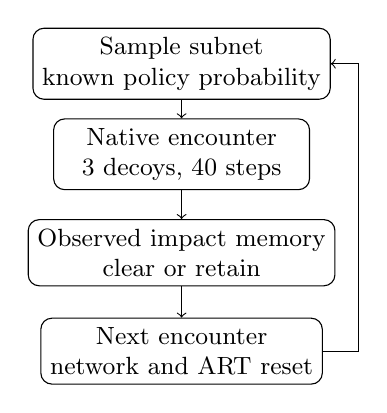
\begin{tikzpicture}[every node/.style={draw,rounded corners,align=center,font=\small,minimum width=3.25cm,minimum height=.65cm}]
\node (p) at (0,0) {Sample subnet\\known policy probability};
\node (e) at (0,-1.15) {Native encounter\\3 decoys, 40 steps};
\node (m) at (0,-2.4) {Observed impact memory\\clear or retain};
\node (r) at (0,-3.65) {Next encounter\\network and ART reset};
\draw[->] (p)--(e);\draw[->] (e)--(m);\draw[->] (m)--(r);
\draw[->] (r.east)--++(.45,0)|-(p.east);
\end{tikzpicture}
\caption{The memory intervention. Protected-server scoring is computed separately from logged impacts; it is not an input to the custom target selector.}
\Description{Four vertically connected boxes show policy sampling, native encounter, observed memory update, and network reset before the next encounter.}
\label{fig:design}
\end{figure}

\section{Estimand and Historical-Data Analysis}
Let $H=8$ encounters form a world initialized with empty memory. For a fixed network and memory law, our target is $V(\pi)=\mathbb{E}_{\pi}[H^{-1}\sum_{t=1}^H R_t]$: deployment of the same candidate from world initialization. It is not the value of switching policies after a particular observed attacker history or forecasting the next real incident.

For logging world $i$, define
\begin{equation}
w_{it}=\prod_{s=1}^{t}\frac{\pi(A_{is})}{\mu(A_{is})},\qquad
\widehat V_{\rm IS}=\frac{1}{nH}\sum_{i=1}^n\sum_{t=1}^H w_{it}R_{it}.
\end{equation}
The prefix includes earlier encounters because their actions can alter retained memory and therefore later outcomes. Under a common transition and memory-update law, matching initial state distribution, known probabilities, and support, ordinary trajectory change of measure applies. Conditioning on complete history can accommodate the memory process; persistence does not by itself make evaluation unidentified. The uniform logger has support for every candidate macro-action.

We also compute the prefix self-normalized estimator
\begin{equation}
\widehat V_{\rm SN}=\frac1H\sum_{t=1}^{H}\frac{\sum_i w_{it}R_{it}}{\sum_i w_{it}},\qquad
N_{{\rm eff},t}=\frac{(\sum_i w_{it})^2}{\sum_i w_{it}^2}.
\end{equation}
Self-normalization has finite-sample bias. IS values need not lie in the outcome range; neither estimator is promoted as novel. A current-encounter ratio diagnostic omits the prefix. With full reset and independent encounter randomness it is a useful simpler estimator; under retained memory it generally evaluates rewards from logging-induced histories rather than the target's lifetime histories. Its performance is descriptive, not a fair test of an algorithm designed for the latter estimand.

We jointly bootstrap 64 logging worlds 1,000 times using seed 20261008. The same resample indices evaluate all candidates within a setting. A candidate is selected only if it has the highest point estimate, wins at least 95\% of bootstrap resamples, and has effective sample size at least 16 at every encounter. Ties split their vote equally. Otherwise the rule abstains. These are prespecified heuristic thresholds, not a confidence bound or calibrated safety guarantee. The bootstrap conditions on the observed log and cannot reveal histories absent from it.

\section{Protocol and Verification}
A 128-world development study on the smaller network preceded validation. Its eight worlds per cell covered reset/retained memory, stable/rotated aliases, and all four policies. Development observations and the earlier analytical toy example are not pooled with validation. The fresh validation protocol and runner were committed before collection; their hashes and the commit are preserved in the freeze record.

Validation crosses two networks, two memory laws, and four policies, with 64 worlds per cell. Logger seeds 30000--30063 and candidate seeds 40000--40063 are disjoint from one another and from development. Candidate policies share seeds to support paired contrasts. Networks and memory settings also share seeds; the two networks are not independent samples from a population of networks. The world, not the step or encounter, is the sampling unit. We report standard errors across worlds and paired standard errors for policy differences. No post hoc sample extension was used.

The run completed all 1,024 attempts without failures in approximately 209 seconds using four local CPU processes. The environment used CPython 3.10.20 and a pinned minimal simulator dependency set, including CPU PyTorch. No HPC allocation or GPU training was needed. This is measured collection time, not installation or analysis time and not a portable performance guarantee.

Independent analysis reconstructs impacts and memory from traces, checks probabilities, action masks, deployment destinations and budgets, and verifies 1,025 input file hashes plus frozen runner, helper, and protocol hashes. A scalar implementation separately reproduces 24 IS/SN estimates. Five deliberately corrupted records test that semantic checks reject altered probability, impacted targets, memory, deployment destination, and outcome, including a resealed trace. Development identity controls compare 64 paired full trajectories. One fresh-process validation-world replay was exactly identical; this is a limited replay check, not an independent laboratory replication.

An exploratory OPEN interface test is retained but excluded from the frozen validation comparison. It did not constitute reproduction of the published experiment: a zero-outcome control produced forecasts deviating from zero by up to about 0.110, while a separate weighted-mean arithmetic control passed. Both the insufficient interface validation and its different forecasting target were recorded before collection. This is not evidence that OPEN's published algorithm fails. The initial simulator import failure and subsequent successful smoke test also remain in the repository.

\section{Results}
\begin{table*}[t]
\centering\small
\setlength{\tabcolsep}{3pt}
\caption{Validation outcomes and offline estimates. Online means use 64 independent worlds per policy within each setting. Current ratio omits previous encounters.}\label{tab:results}
\begin{tabular}{rlcrrrrr}\toprule
Hosts & Memory & Policy & Online & SE & Prefix IS & Prefix SN & Current ratio\\ \midrule
15 & Reset & D & 0.6602 & 0.0133 & 0.7486 & 0.6453 & 0.7020 \\
15 & Reset & S & 0.5848 & 0.0128 & 0.5392 & 0.6009 & 0.5721 \\
15 & Reset & U & 0.5559 & 0.0165 & 0.5152 & 0.5855 & 0.5716 \\
15 & Retained & D & 0.3711 & 0.0142 & 0.4504 & 0.3972 & 0.4198 \\
15 & Retained & S & 0.3613 & 0.0126 & 0.3244 & 0.3510 & 0.3513 \\
15 & Retained & U & 0.4430 & 0.0168 & 0.3621 & 0.4060 & 0.4090 \\
25 & Reset & D & 0.8619 & 0.0065 & 1.0093 & 0.8726 & 0.9034 \\
25 & Reset & S & 0.8357 & 0.0059 & 0.7377 & 0.8172 & 0.8059 \\
25 & Reset & U & 0.8244 & 0.0065 & 0.7491 & 0.8486 & 0.8366 \\
25 & Retained & D & 0.7199 & 0.0103 & 0.8861 & 0.7687 & 0.7991 \\
25 & Retained & S & 0.7373 & 0.0096 & 0.6677 & 0.7374 & 0.7136 \\
25 & Retained & U & 0.7658 & 0.0106 & 0.6963 & 0.7859 & 0.7649 \\
\bottomrule\end{tabular}
\end{table*}
Table~\ref{tab:results} reports every candidate. In both network configurations the highest online mean changes from D under reset memory to U under retained memory. The paired D-minus-U contrast changes sign in both cases (Table~\ref{tab:contrasts}). Those finite-world differences support a memory-sensitive ranking in this testbed; they do not identify a universally preferred deployment location. Lower-ranked policies can be close, and their ordering should not be overinterpreted.

\begin{table}[t]
\centering\small
\setlength{\tabcolsep}{3pt}
\caption{Paired D-minus-U contrasts. Positive values favor D; negative values favor U.}\label{tab:contrasts}
\begin{tabular}{rlrr}\toprule
Hosts & Memory & D minus U & Paired SE\\ \midrule
15 & Reset & 0.1043 & 0.0139 \\
15 & Retained & -0.0719 & 0.0170 \\
25 & Reset & 0.0375 & 0.0056 \\
25 & Retained & -0.0459 & 0.0096 \\
\bottomrule\end{tabular}
\end{table}
\begin{figure*}[t]\centering
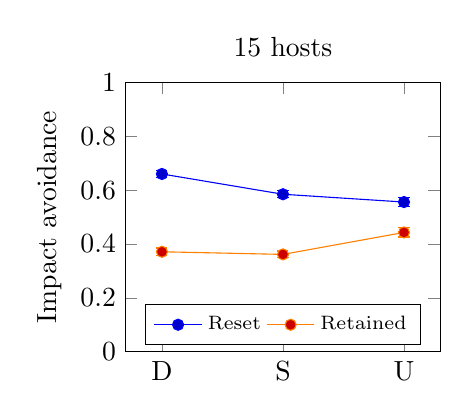
\begin{tikzpicture}\begin{axis}[width=.46\textwidth,height=5cm,ymin=0,ymax=1,xmin=.7,xmax=3.3,xtick={1,2,3},xticklabels={D,S,U},ylabel={Impact avoidance},title={15 hosts},legend style={font=\scriptsize,at={(.5,.1)},anchor=center},legend columns=2]
\addplot+[color=blue,mark=*,error bars/.cd,y dir=both,y explicit] coordinates {(1,0.66015625) +- (0,0.01329000) (2,0.58476562) +- (0,0.01282583) (3,0.55585938) +- (0,0.01646777)};
\addplot+[color=orange,mark=*,error bars/.cd,y dir=both,y explicit] coordinates {(1,0.37109375) +- (0,0.01423063) (2,0.36132812) +- (0,0.01257332) (3,0.44296875) +- (0,0.01683756)};\legend{Reset,Retained}\end{axis}\end{tikzpicture}\hfill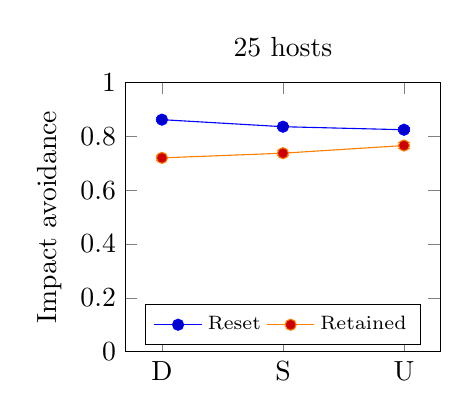
\begin{tikzpicture}\begin{axis}[width=.46\textwidth,height=5cm,ymin=0,ymax=1,xmin=.7,xmax=3.3,xtick={1,2,3},xticklabels={D,S,U},ylabel={Impact avoidance},title={25 hosts},legend style={font=\scriptsize,at={(.5,.1)},anchor=center},legend columns=2]
\addplot+[color=blue,mark=*,error bars/.cd,y dir=both,y explicit] coordinates {(1,0.86191406) +- (0,0.00647194) (2,0.83574219) +- (0,0.00585208) (3,0.82441406) +- (0,0.00651966)};
\addplot+[color=orange,mark=*,error bars/.cd,y dir=both,y explicit] coordinates {(1,0.71992188) +- (0,0.01028834) (2,0.73730469) +- (0,0.00958549) (3,0.76582031) +- (0,0.01063113)};\legend{Reset,Retained}\end{axis}\end{tikzpicture}\caption{Online means with one world-level standard error. Policies favor DMZ (D), server (S), or user (U) placement. Lines connect policies for readability, not interpolation.}\Description{Two panels show higher impact avoidance with reset memory and a change from D to U as the leading policy when memory is retained.}\label{fig:outcomes}\end{figure*}
Figure~\ref{fig:outcomes} displays the online means with one standard error. Retaining memory reduces the outcome for every policy in these configurations. The comparator is the same wrapper with inter-encounter memory cleared, not an unrelated stronger attacker. Nevertheless, the change is conditional on stable original identifiers and the chosen prioritization rule.

\begin{table*}[t]
\centering\small
\setlength{\tabcolsep}{3pt}
\caption{Predeclared decision diagnostic. Thresholds: winner frequency at least 0.95 and every encounter ESS at least 16.}\label{tab:decisions}
\begin{tabular}{rlcrrl}\toprule
Hosts & Memory & Top & Frequency & Min ESS & Decision\\ \midrule
15 & Reset & D & 0.974 & 15.68 & Abstain \\
15 & Retained & U & 0.552 & 15.48 & Abstain \\
25 & Reset & D & 0.976 & 15.68 & Abstain \\
25 & Retained & U & 0.844 & 15.48 & Abstain \\
\bottomrule\end{tabular}
\end{table*}
The highest prefix-SN estimate matches the highest observed online mean in all four settings. This should not be read as a measured 100\% selection reliability: there are only four deliberately related settings, and each uses one logging dataset. The offline order among lower-ranked candidates does not always match the online order. Estimation errors and the history-discarding diagnostic are fully reported rather than selecting the best-looking estimator after collection.

The decision rule abstains in all four settings (Table~\ref{tab:decisions}). Under reset memory, bootstrap winner frequency exceeds the threshold but minimum effective sample size does not. Under retained memory, winner frequency also falls short. Effective sample sizes are the same across networks and memory laws for a fixed candidate because the action generator, logger seeds, and probabilities are shared. This is an expected design property, not independent corroboration.

The all-abstain result does not validate the threshold as a useful deployment rule. A trivially conservative rule can avoid every selection error by making no decisions. Here it serves to expose the difference between a point-estimate ranking and sufficient evidence under a declared heuristic. Evaluating coverage, regret, and decision frequency across independent logging datasets would be required to establish utility.

\section{Discussion and Limitations}
The strongest supported finding is that a small change in evaluation state continuity changes the leading policy in two supplied networks, with a trace-audited explanation of what is carried forward. This argues for reporting attacker reset semantics alongside cyber-defense performance. It does not establish that the added memory rule resembles human expertise, learns deception recognition, or is stronger than published adaptive adversaries.

The corpus supports methodological research because historical probabilities and corresponding online references are both available. However, its narrow action space, short horizon, equal deployment budgets, and small supplied topologies limit generalization. We do not test learned defenses, alternative memory decay, adversarial manipulation of logs, costs of relocating assets, uncertain impact observations, or out-of-distribution production traffic. Rotated aliases are only a development diagnostic. Larger networks alone would not resolve these limitations.

The study observes one finite logging sample per setting. Bootstrap intervals describe resampling that sample; they do not establish across-dataset coverage or quantify simulator-model error. Prefix weighting can lose efficiency as the horizon grows even when support holds. The threshold of 16 lies close to the observed minimum for the winning reset policy, so its abstention is sensitive to that engineering choice. The threshold was fixed before validation, but that fact does not make it optimal.

Current-encounter weighting is particularly relevant in the reset setting, where carrying prefix ratios adds unnecessary variance. A future estimator comparison should include this setting-specific baseline explicitly and compare efficient history-aware alternatives under retained memory. No conclusion here supports universal superiority of prefix SN over other estimators. OPEN, regression-assisted DR, and strategic-response methods require matched estimands, assumptions, and validated implementations before comparison.

The initial feasibility plan sought broader comparator reproduction and full-text overlap review. These gates were not fully met: CoADAM full text remained inaccessible and OPEN interface reproduction remained insufficient. The validation proceeded as a bounded artifact investigation with these limitations disclosed, not as clearance for an algorithmic novelty claim. The draft therefore should not be submitted as evidence of a new general OPE method. A broader benchmark contribution needs independent users, multiple attacker families, and repeated logging datasets before journal suitability can be responsibly asserted.

\section{Conclusion}
In a fixed simulator experiment, retained target memory reverses the leading deception-placement policy on two supplied networks. The historical-data point estimates recover the observed leaders, yet a predeclared evidence heuristic abstains throughout. The release makes this distinction inspectable through complete propensities, memory transitions, outcomes, and verification code. Its value is a reproducible empirical case and a benchmark starting point, bounded by one memory heuristic and a small policy family.

\section*{Artifact, Ethics, and Author Review}
Code, generated traces, protocols, failures, and validation records are available at \url{https://github.com/ezekielologunde/adaptive-deception-evaluation}. No confidential traffic or human participant data are used. Cyberwheel is obtained from its pinned MIT-licensed upstream source; other inspected artifacts retain their own terms. Original project material is intentionally unlicensed pending the author's decision. The experiment executes simulator actions only.

This manuscript was prepared with AI-assisted coding, analysis, and drafting. Automated checks are not an independent investigator's replication. The named author must review and take responsibility for the scientific claims, citations, and applicable venue disclosure requirements before submission. No submission, acceptance, external funding, or institutional affiliation is asserted.

\begin{thebibliography}{9}
\bibitem{open} Yash Chandak, Shiv Shankar, Nathaniel D. Bastian, Bruno Castro da Silva, Emma Brunskill, and Philip S. Thomas. 2022. Off-Policy Evaluation for Action-Dependent Non-Stationary Environments. NeurIPS. \url{https://proceedings.neurips.cc/paper_files/paper/2022/file/3bf80b34f731313b8292f4578e820c90-Paper-Conference.pdf}
\bibitem{liu} Vincent Liu, Yash Chandak, Philip Thomas, and Martha White. 2023. Asymptotically Unbiased Off-Policy Policy Evaluation when Reusing Old Data in Nonstationary Environments. AISTATS, PMLR 206, 5474--5492. \url{https://proceedings.mlr.press/v206/liu23d.html}
\bibitem{vo} Kiet Q. H. Vo, Abbavaram Gowtham Reddy, Julian Rodemann, Siu Lun Chau, and Krikamol Muandet. 2026. Off-Policy Evaluation with Strategic Agents via Local Disclosure. ICML, PMLR 306, 124108--124127. \url{https://proceedings.mlr.press/v306/vo26b.html}
\bibitem{safe} Shayan Doroudi, Philip S. Thomas, and Emma Brunskill. 2017. Importance Sampling for Fair Policy Selection. UAI. \url{https://cs.stanford.edu/people/ebrun/pdfs/doroudi2017uai.pdf}
\bibitem{cyberwheel} ORNL. Cyberwheel source repository. Revision 6e535b50eea991ed48bb9eeb46b4b267090cc897, accessed October 7, 2026. \url{https://github.com/ORNL/cyberwheel}
\bibitem{trident} Ryozo Masukawa, Ian Bryant, Armita Kazeminajafabadi, Sanggeon Yun, Hyunwoo Oh, SungHeon Jeong, Nathaniel D. Bastian, Mahdi Imani, and Mohsen Imani. 2026. Trident: How to Break Deep Reinforcement Learning Cyber Defenses (Agentic). arXiv:2608.04317v1, preprint. \url{https://arxiv.org/html/2608.04317v1}
\bibitem{coadam} CoADAM source repository. 2026. Revision 69defb709190547c99ff54ca4f9fb6ade7e510d6. Baseline comparison source, accessed October 7, 2026. \url{https://github.com/Usmanjibril09/CoADAM}
\end{thebibliography}
\end{document}
